\documentclass[11pt]{article}
\usepackage{geometry}                
\geometry{letterpaper}                   

\usepackage{graphicx}
\usepackage{amssymb}
\usepackage{epstopdf}
%\usepackage{natbib}
\usepackage{amssymb, amsmath}
\DeclareGraphicsRule{.tif}{png}{.png}{`convert #1 `dirname #1`/`basename #1 .tif`.png}

\usepackage{listings}
\usepackage{color} %red, green, blue, yellow, cyan, magenta, black, white
\definecolor{mygreen}{RGB}{28,172,0} % color values Red, Green, Blue
\definecolor{mylilas}{RGB}{170,55,241}

%\title{Zurich traffic simulation Sihlstrasse/Uraniastrasse}
%\author{Filip Meier, Sebastian Honegger}
%\date{date} 

\begin{document}



\thispagestyle{empty}

\begin{center}
\includegraphics[width=5cm]{ETHlogo.eps}

\bigskip


\bigskip


\bigskip


\LARGE{ 	Lecture with Computer Exercises:\\ }
\LARGE{ Modelling and Simulating Social Systems with MATLAB\\}

\bigskip

\bigskip

\small{Project Report}\\

\bigskip

\bigskip

\bigskip

\bigskip


\begin{tabular}{|c|}
\hline
\\
\textbf{\LARGE{Zurich traffic simulation Sihlstrasse/Uraniastrasse}}\\
\\
\hline
\end{tabular}
\bigskip

\bigskip

\bigskip

\LARGE{Filip Meier \& Sebastian Honegger}



\bigskip

\bigskip

\bigskip

\bigskip

\bigskip

\bigskip

\bigskip

\bigskip

Zurich\\
December 2015\\

\end{center}



\newpage

%%%%%%%%%%%%%%%%%%%%%%%%%%%%%%%%%%%%%%%%%%%%%%%%%

\newpage
\section*{Agreement for free-download}
\bigskip


\bigskip


\large We hereby agree to make our source code for this project freely available for download from the web pages of the SOMS chair. Furthermore, we assure that all source code is written by ourselves and is not violating any copyright restrictions.

\begin{center}

\bigskip


\bigskip


\begin{tabular}{@{}p{3.3cm}@{}p{6cm}@{}@{}p{6cm}@{}}
\begin{minipage}{3cm}

\end{minipage}
&
\begin{minipage}{6cm}
\vspace{2mm} \large Filip Meier

 \vspace{\baselineskip}

\end{minipage}
&
\begin{minipage}{6cm}

\large Sebastian Honegger

\end{minipage}
\end{tabular}


\end{center}
\newpage

%%%%%%%%%%%%%%%%%%%%%%%%%%%%%%%%%%%%%%%



% IMPORTANT
% you MUST include the ETH declaration of originality here; it is available for download on the course website or at http://www.ethz.ch/faculty/exams/plagiarism/index_EN; it can be printed as pdf and should be filled out in handwriting


%%%%%%%%%% Table of content %%%%%%%%%%%%%%%%%

\tableofcontents

\newpage

%%%%%%%%%%%%%%%%%%%%%%%%%%%%%%%%%%%%%%%



\section{Abstract}

The following report shows a simulation for a specific street in Zurich (Uraniastrasse/Sihlstrasse) which should be changed in the future to a pedestrian area (Sihlstrasse). The simulation is implemented with MATLAB and we used the \textit{Nagel-Schreckenber-model} as the basic simulation model. To implement the traffic lights for city traffic we used finally the  \textit{Chowdhury-Schadschneider-Model}. The results for the traffic jam in the neighbourhood is much higher than today. We get traffic jam value which are up to 6 times higher than today.

\section{Individual contributions}

In our project, both of us were active and contributed in the development of the simulation. We worked together at the program and at the report.

\section{Introduction and Motivations}


The city of Zurich planing to change one specific part of the Sihlstrasse in a pedestrian area. The idea is to make this area more comfortable for the visitors of the city center and it should be also an upgrade for the restaurants and shops around this area.
\begin{figure}[h]
\begin{minipage}[t]{.45\textwidth}
	\centering
	\vspace{30pt}
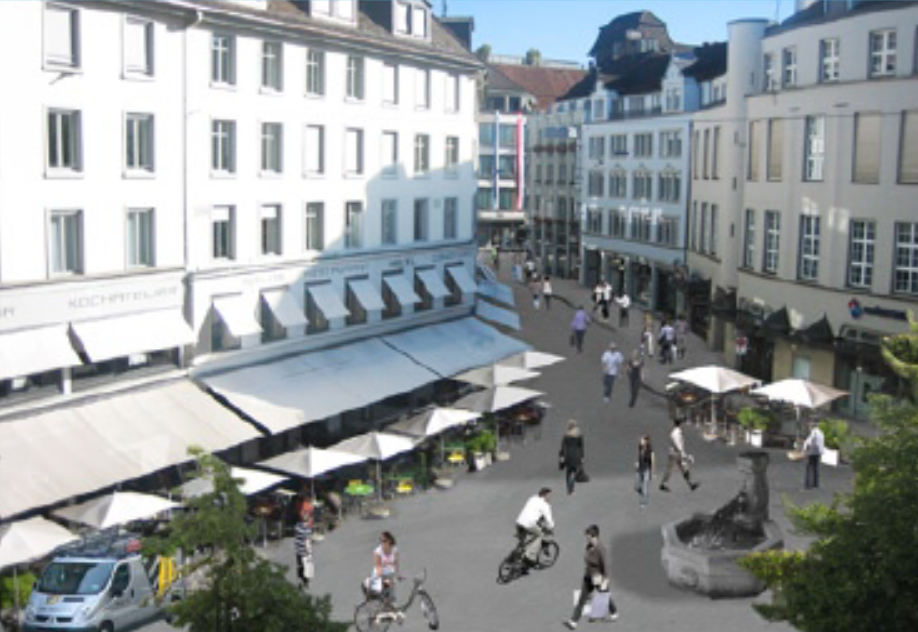
\includegraphics[width=\textwidth]{pedestrianarea.png}
\end{minipage}\hfill
\begin{minipage}[t]{.45\textwidth}
	\centering
	\vspace{0pt}
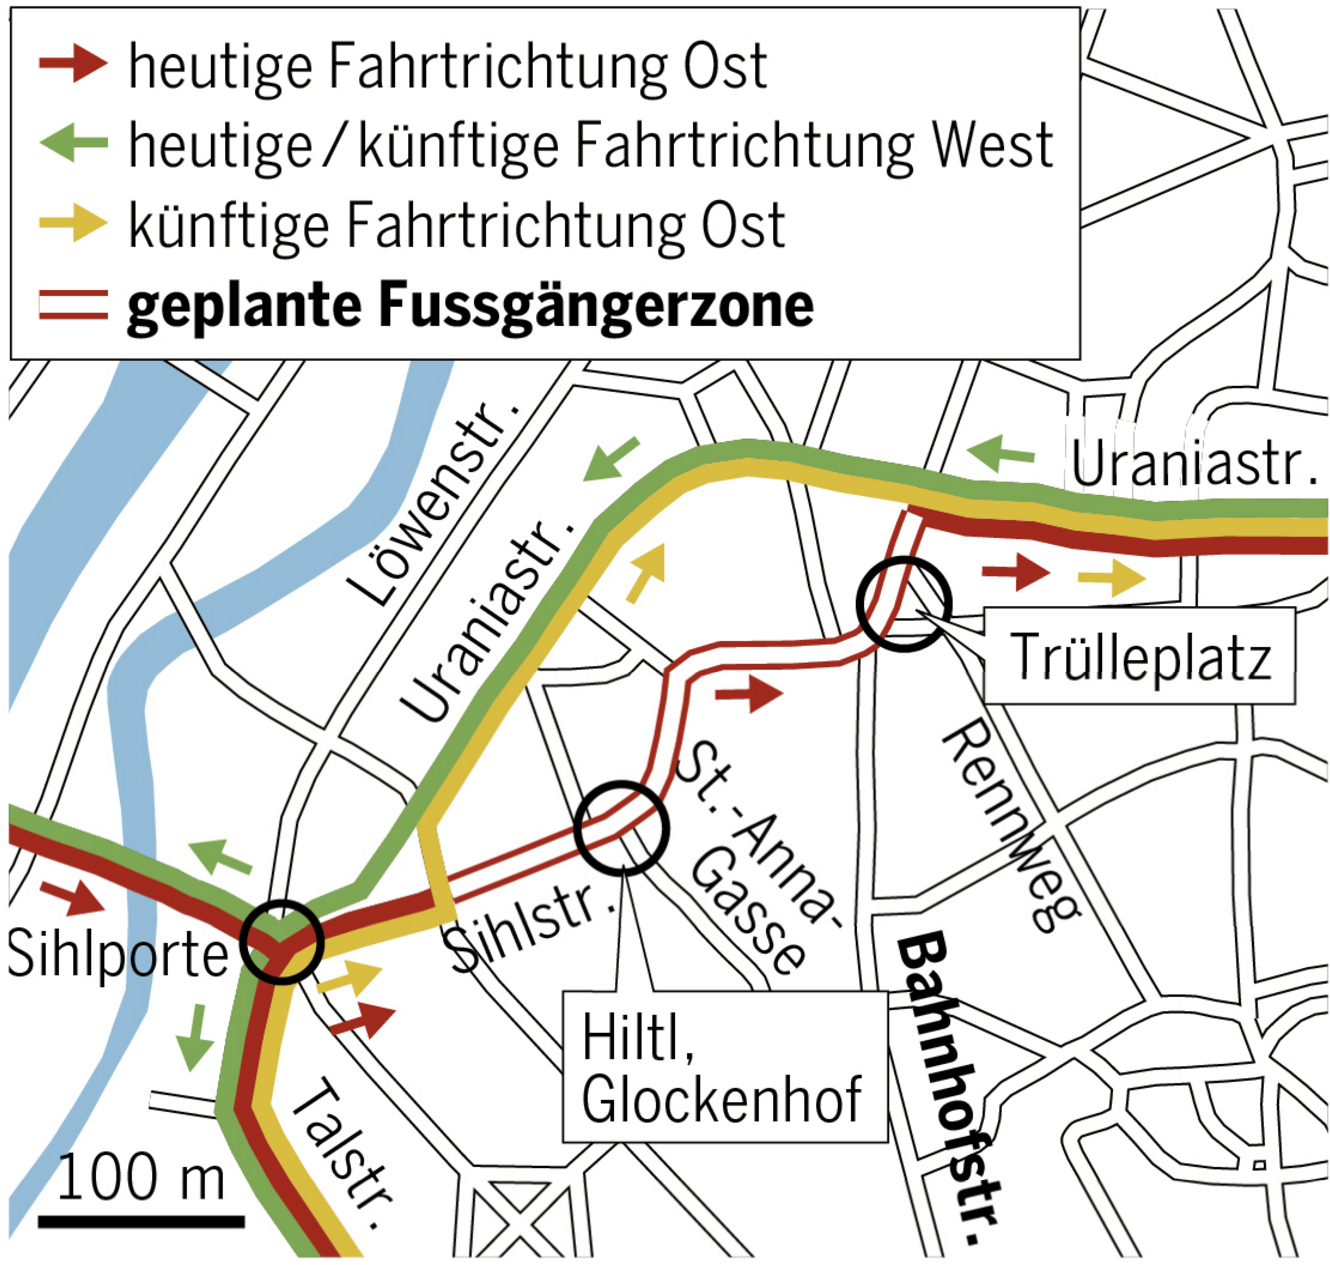
\includegraphics[width=\textwidth]{Plan_Sihlstrasse.png}
\end{minipage}\hfill
\caption{right: situation plan which shows the change of the tracks. left: illustraion of the pedestrian area at sihlstrasse.\cite{project}}
\end{figure}
\\
The change will have a big impact for the traffic because there will be one lane less than before. Sihlstrasse (from west to east) and Uraniastrasse (from east to west) is one of the most travelled  road in the city center. It is the only alternative road to the highway (Westumfarung). If they decide to built a pedestrian area in the Sihlstrasse they will lose one track from west to east\cite{project}.
We know want to analyse the impact to the traffic jam and the impact on the neighbourhood streets.

\section{Fundamental Questions}

With our simulation, we want to answered the following questions:
\begin{itemize}
\item[1.] Are the streets still large enough to manage the traffic jam peaks on working days?
\item[2.] What is the impact on the neigbourhood streets?

\end{itemize}
\section{Description of the Model}

\subsection{Nagel-Schreckenberg-model}

Our model is based on the prototype of cellular automata model which is called \textit{Nagel-Schreckenber-model}. It was developed by Kai Nagel and Michael Schreckenberg in 1992. The basic idea was to split the streets in cells, which contain only one car. Therefore we can identify on cell with the typical required space for one car in a traffic jam. Generally this length is around $7.5\,\mathrm{m}$, which correspond approximately the length of the car and the average distance to the car in front in a traffic jam.
\begin{figure}[h!]
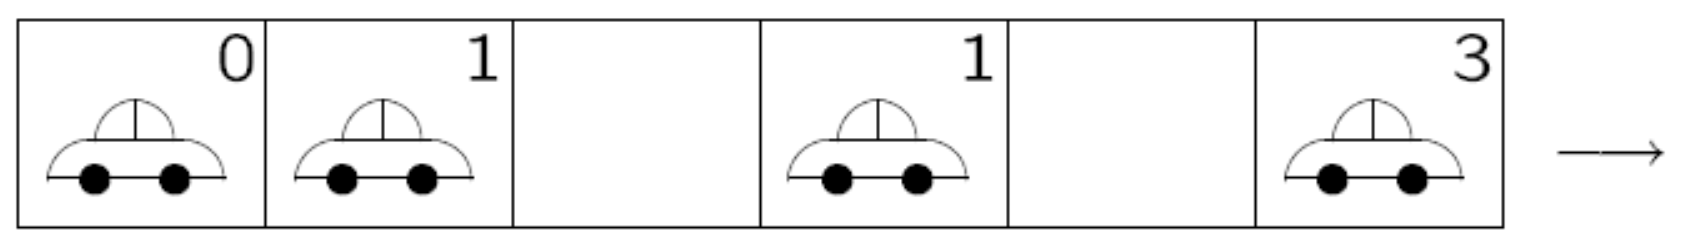
\includegraphics[width=\textwidth]{ns_config.png}
\caption{this figure illustrate the typical \textit{Nagel-Schreckenberg-model} configuration: one cell (approx. $7.5\,\mathrm{m}$) which can include exactly one car.\cite{theory}}
\label{ns_config} 
\end{figure}
Figure (\ref{ns_config}) shows a typical \textit{Nagel-Schreckenberg-model} set-up, one cell (approx. $7.5\,\mathrm{m}$) which include one car. The number in the upper right corner of the cell (which include a car) representing the actual velocity $v_n$ of the car $n$. The velocity is a discrete value an we assume that the car $n$ can have the velocities $v_n=0,1 \ldots ,v_{\mathrm{max}}$. Every car has the same $v_{\mathrm{max}}$ which has the same effect like a speed limit.\\
With this properties one have a good description of the state of the street at time $t$. The next step is to define the development in time. So we have to define the state of the street at the time $t+1$. To simulate this time step in the \textit{Nagel-Schreckenberg-model} we have to define for steps, which we have to apply for each car $n$:
\begin{itemize}
\item[1.]	\textbf{Acceleration}\\
\\
If $v_n<v_{\mathrm{max}}$ at time $t$, the car $n$ will accelerate is velocity about one unit:
\begin{equation}
v_n \rightarrow v'_n = \min(v_n+1,v_\mathrm{max})
\label{accel}
\end{equation}
$v'_n$ represents the new velocity at time $t+1$.
\item[2.]  \textbf{Slow down}\\
\\
We define $d_n$ as the number of empty cells in front of the car $n$ until to the next car $n+1$. So if $d_n$ is smaller than $v'_n$, the car $n$ has to slow down to the velocity $d_n$:
\begin{equation}
v'_n \rightarrow v''_n = \min(v_n',d_n)
\label{slowd}
\end{equation}
\item[3.]  \textbf{Randomization}\\
\\
If $v''_n>0$, the velocity of car $n$ will be randomly with the probability $p$ reduced about one unit:
\begin{equation}
v''_n \rightarrow v'''_n=
\begin{cases}
\max(v''_n-1,0) & \mathrm{with\,probability} \quad p\\
v''_n & \mathrm{with\,probability} \quad 1-p
\end{cases}
\label{hangbb}
\end{equation}
\item[4.] \textbf{Drive}\\
\\
The car $n$ drives with the new velocity $v_n(t+1)=v'''_n$ about $v_n(t+1)$ cells:
\begin{equation}
x_n(t+1)=x_n(t)+v_n(t+1)
\label{drive}
\end{equation}
\end{itemize}
One have to apply every step simultaneous to every car. So we can not simulate the real situation, that the car in front can move as well simultaneous to the car behind.
\\
One can see that just step (\ref{slowd}) has a interaction between cars and with step (\ref{hangbb}) the simulations has a stochastic  dynamic. Therefore the \textit{Nagel-Schreckenberg-model} is called a stochastic cellular automata.\\
\begin{figure}[h!]
\begin{itemize}
\item[1.] \textbf{start configuration} \\
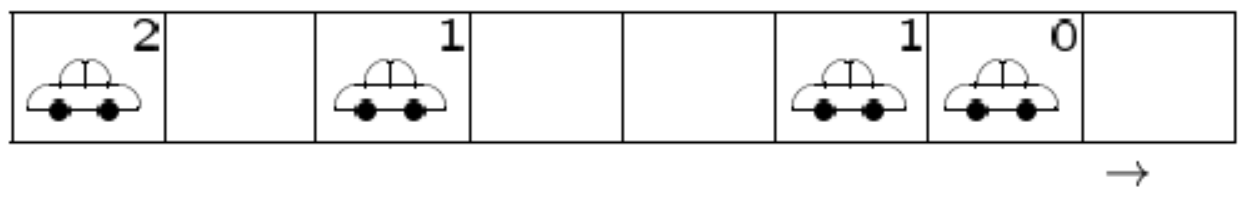
\includegraphics[width=\textwidth]{config_1.png}
\item[2.] \textbf{acceleration} ($v_{\mathrm{max}}=2$) \\
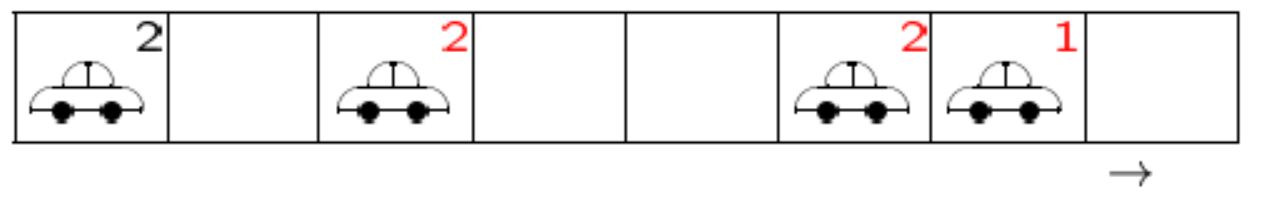
\includegraphics[width=\textwidth]{config_2.png}
\item[3.] \textbf{slow down} \\
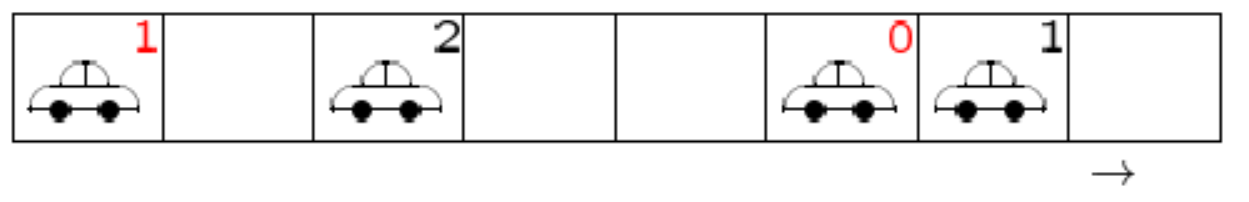
\includegraphics[width=\textwidth]{config_3.png}
\item[4.] \textbf{Randomization} ($p=\frac{1}{3}$) \\
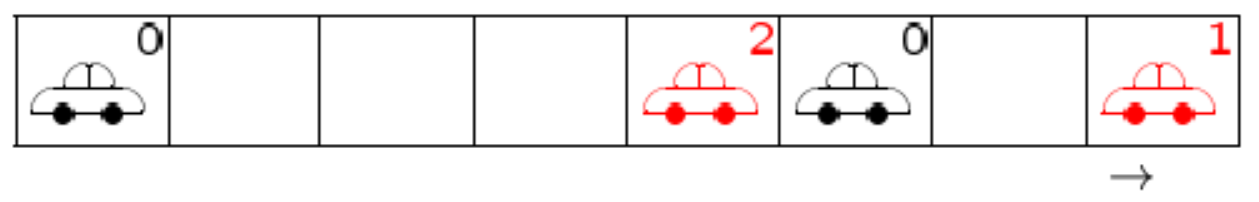
\includegraphics[width=\textwidth]{config_4.png}
\item[5.] \textbf{drive} ($=$ configuration at $t+1$) \\
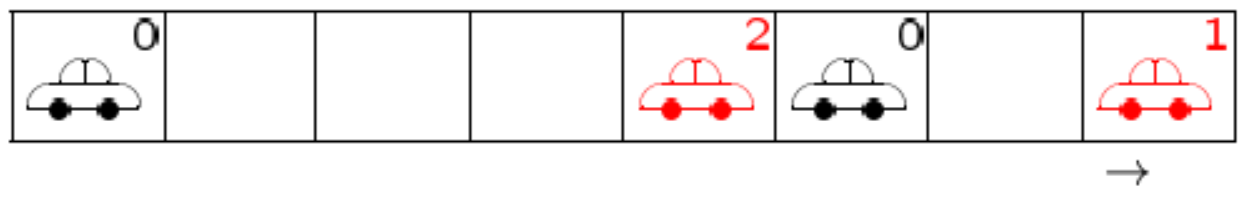
\includegraphics[width=\textwidth]{config_5.png}
\end{itemize}
\caption{Shows on complete time step of the \textit{Nagel-Schreckenberg-model} with acceleration, slow down, hang behind probability and drive.}
\label{example_ns} 
\end{figure}\\
Figure (\ref{example_ns}) shows a complete time step of the \textit{Nagel-Schreckenberg-model}. In this case in step 4 we have three car which are able to hang behind but just one will to it in the next step (probability $p=\frac{1}{3}$). And as one can see the speed limit in this example is $v_\mathrm{max}=2$.
\begin{itemize}
\item[1.] The first step in figure \ref{example_ns} shows that all cars want to accelerate as soon as possible to maximum speed limit.
\item[2.] the 'slow down' step (figure \ref{example_ns}) prevent car accidents. But as mention before it does not include the movement of the car in front at the same time.
\item[3.] The step Randomization simulates different effects. It tries to modelling for example natural fluctuations in driving style. A normal car drives never with a total constant speed it always fluctuate between $v_\mathrm{max}$ und $v_\mathrm{max}-1$. This function generates an asymmetry for the acceleration and the slow down mode. In detail it will generate a stronger slow down and sometimes the speed stays constant instead to accelerate. If we have a high density of cars, the above described effects could have a traffic jam as result.
\item[4.] The last step is just the motion of the cars with the new speed which is compute with the steps 1 to 3.

\end{itemize}
We already defined the length of one cell ($7.5\,\mathrm{m}$) but we also have to define the correct time scale for one time step $t$ $\rightarrow$ $t+1$. Therefore we need a value for the average speed, one can calculate it in the following way:\\

\begin{equation}
v_\mathrm{aver}=(1-p)v_\mathrm{max} + p(v_\mathrm{max}-1)=v_\mathrm{max}-p
\label{average_speed}
\end{equation}
We now identify this speed with $50\,\mathrm{km/h}$. For a model with $v_\mathrm{max}=5$ and $p=0.5$ we get\\
\begin{equation}
\frac{7.5\,\mathrm{m}}{\mathrm{cells}}\cdot\frac{4.5\,\mathrm{cells}}{\mathrm{timestep}} \cdot \frac{3.6\,\mathrm{s}}{50\,\mathrm{m}}\approx 2.5\,\frac{\mathrm{s}}{\mathrm{timestep}}
\label{time}
\end{equation}

\subsection{Chowdhury-Schadschneider-Modell}

The dynamic of a real city traffic is characterized through the interaction of two time scales, the driving time between two traffic lights and the time of the green phase of each traffic light. Chowdhury and Schadschneider have modify the \textit{Nagel-Schreckenberg-model} with a algorithm for traffic lights to simulate the traffic of a city. The dynamic is define by the following steps. $d_n$ define as before the gap to the next car and $s_n$ defines the distance to the next traffic light:\\

\begin{itemize}
\item[1.]	\textbf{Acceleration}\\
\\
If $v_n<v_{\mathrm{max}}$ at time $t$, the car $n$ will accelerate is velocity about one unit:
\begin{equation}
v_n \rightarrow v'_n = \min(v_n+1,v_\mathrm{max})
\label{accel_t}
\end{equation}
$v'_n$ represents the new velocity at time $t+1$.
\item[2.]  \textbf{Slow down because of cars or traffic lights}\\
\\
\begin{itemize}
\item[1.]case: The traffic light is red:
\begin{equation}
v'_n \rightarrow \min(v_n,d_n,s_n)
\end{equation}
\item[2.]case: The traffic light is green:
\begin{itemize}
\item[a.] The traffic light get red in the next time step:
\begin{equation}
v'_n \rightarrow \min(v_n,d_n,s_n)
\label{min_lights}
\end{equation}
\item[b.] The traffic light is not getting red:
\begin{equation}
v'_n \rightarrow \min(v_n,d_n)
\end{equation}
\end{itemize}

\end{itemize}
\item[3.]  \textbf{Randomization}\\
\\
If $v''_n>0$, the velocity of car $n$ will be randomly with the probability $p$ reduced about one unit:
\begin{equation}
v''_n \rightarrow v'''_n=
\begin{cases}
\max(v''_n-1,0) & \mathrm{with\,probability} \quad p\\
v''_n & \mathrm{with\,probability} \quad 1-p
\end{cases}
\label{hangb}
\end{equation}
\item[4.] \textbf{Drive}\\
\\
The car $n$ drives with the new velocity $v_n(t+1)=v'''_n$ about $v_n(t+1)$ cells:
\begin{equation}
x_n(t+1)=x_n(t)+v_n(t+1)
\label{drive}
\end{equation}
\end{itemize}
The simulations is exactly like the \textit{Nagel-Schreckenberg-model} just the interaction with the traffic lights in step 2 is new. If we have a red traffic light the has to stop before. Therefore the velocity $v_n$ of car $n$ should not be higher then the distance $s_n$ to the next traffic light. So the car will be affected by the traffic light if $s_n<v_n$.\\
If the traffic light is green we can simulate a kind of orange phase. If the traffic light gets red in the next step, the cars will slow down immediately. If the traffic light not get red the simulation will just look on the distance to the next car.

\section{Implementation}

\subsection{Main simulation}

In the main script we define all global parameter: time steps and $v_\mathrm{max}$. Then we have to define the streets for each direction through an array. One cell represents around $7.5\,\mathrm{m}$ and can be occupied only by one car. We then define the location of the cells where the traffic lights are placed. Therefore we used a second array which has the information of the location for the different traffic lights and the current status (green or red). We measured the whole street and the locations of the traffic lights in google maps.\\
For convenience we neglected several small cross streets around the area of sihlstrasse and uraniastrasse.\\
To simulate one hour we call different functions in a loop. The important ones are the following:

\begin{itemize}
\item[1.] We apply the \textit{Chowdhury-Schadschneider-Model} for the current street status.
\item[2.] We add cars on the beginning of the street. Therefore we use an algorithm which works like a traffic light.
\item[3.] We take the cars away from the street at the end of it. We also use an algorithm which works like a traffic light.
\item[4.] To keep the actual status of the street, we add it in a matrix.
\end{itemize}  
In figure \ref{carfigure} you will see an visualization of this process in form of matrix. Figure \ref{carfigure} shows the current status with two lanes in each direction. The more redish cars are the fast ones and the more yellow cars are the slow ones and the black cars have no movement at the moment. The upper figure has time axis from top to bottom and the street from right to left. And the one above has time axis from top to bottom and the street from left to right.
\newpage
\begin{figure}[h!]
	\centering
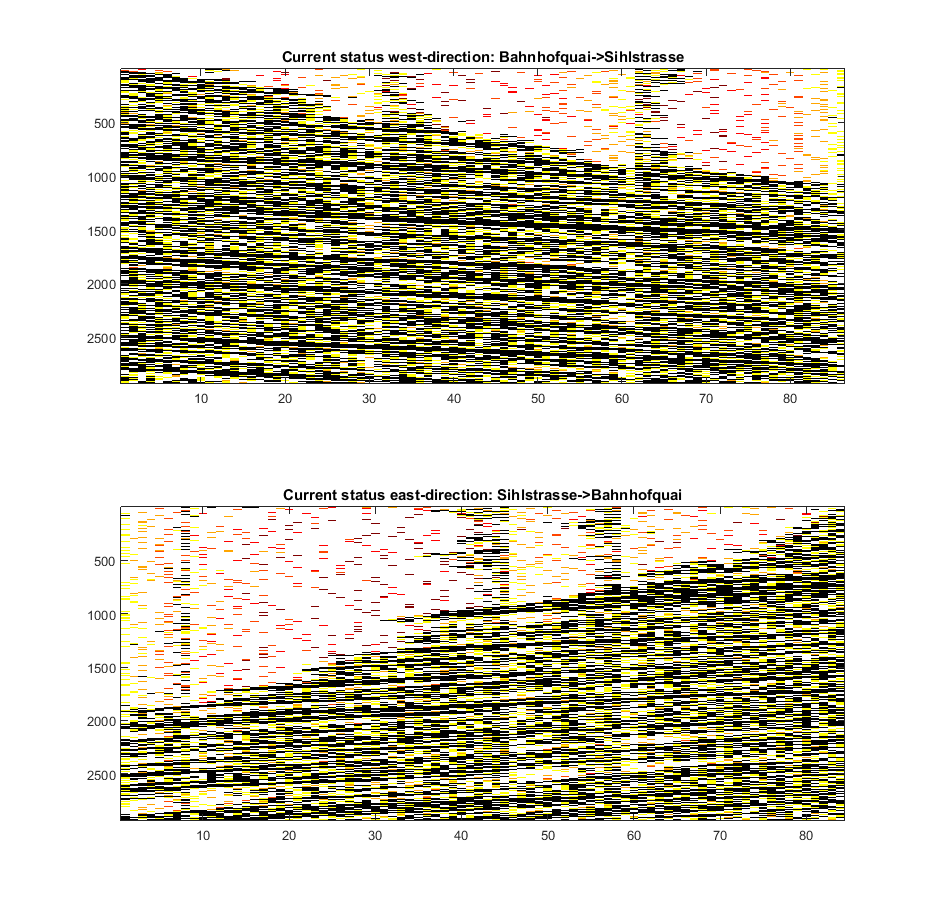
\includegraphics[width=\textwidth]{Current_6pm.png}
\caption{Visualization over a long duration (1h) of the two lane street (current status) in both directions around 6pm. The timesteps from top to the bottom are $2.5\,\mathrm{s}$. The $x$-axis represents the streets. }
\label{carfigure}
\end{figure}

\subsection{Chowdhury-Schadschneider-Model-implementation}
For the different steps in the \textit{Nagel-Schreckenberg-model} we defined one function for each step, figure \ref{accel} for example shows the acceleration function.\\
For this function we just use the minima function of matlab. Input is the current velocity $v_n$ of the car and the maximum velocity $v_\mathrm{max}$.
\\
The most difficult function is the slow down function were we have to implement the two slow down reasons: the next traffic light or the next car. For the distance to the next car $d_n$ we defined first $d_n=0$ and then we implemented a loop over the length of the whole street to check where the next car is located.\\
For the traffic lights we made in a similar way. First of all we have to check which traffic light is the next one in front of the car. Then we can analyse the traffic light: is it currently green or red and is it going to be red in the next step. If it is green we can ignore it, therefore we set $s_n$ , which is the distance to the next traffic light, to a high value. Like this it will not influence the car in the next time steps. If it is red we have to compute the exact value for $s_n$.\\
Finally we get the values for $d_n$ and $s_n$. Now we just can define the minima of $v_n$, $d_n$ and $s_n$ as mention in equation \ref{min_lights}. This will be the value of our output of the slow down function.\\
For the probability function we used simply the function rand from matlab, which define randomly a number between $0$ and $1$ and then we just can define a probability $p$ and an if command.\\



\section{Simulation Results and Discussion}

We simulated first of all the current status of the street. The city of zurich \cite{tief1} sent us data of the average traffic for 24 hours. With our simulation we now can determine the traffic jam ahead the first traffic light. Figure \ref{traffic24_2_lane} shows the traffic jam in cars per unit. As you can see at the typically traffic jam hours (morning time and evening time) we got peak-values of traffic jam.\\
\begin{figure}[h!]
	\centering
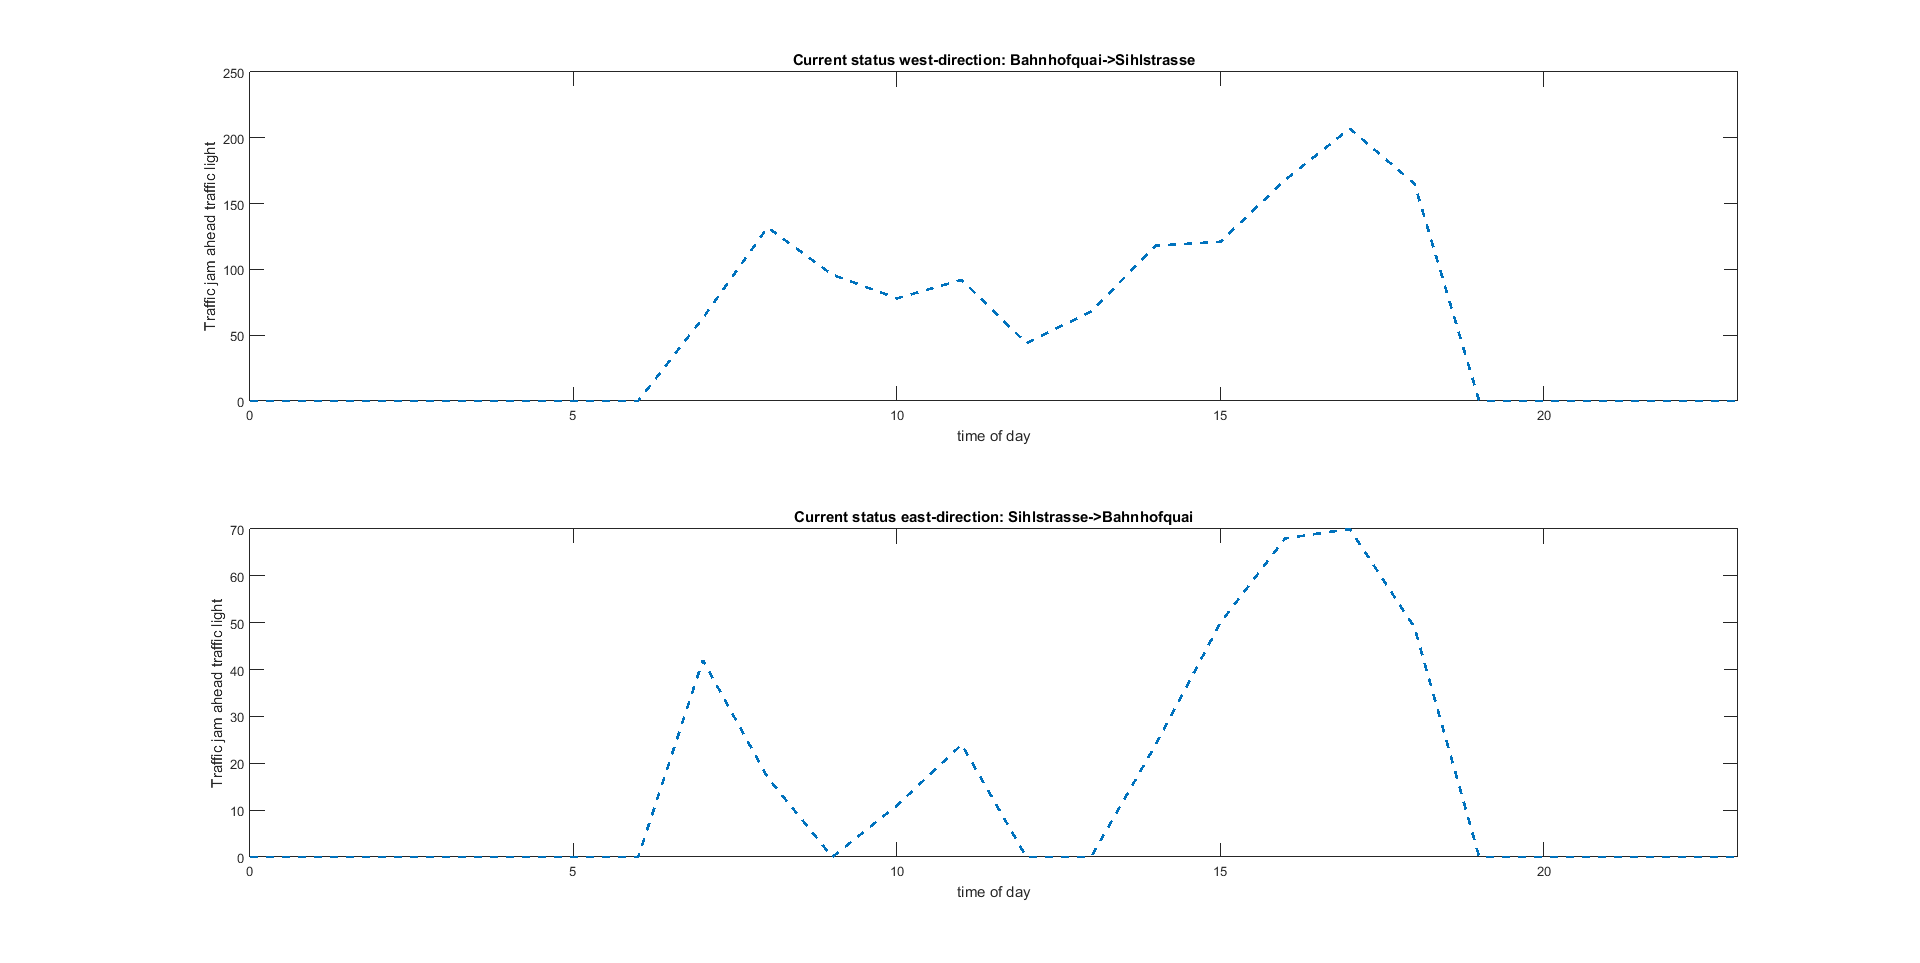
\includegraphics[width=\textwidth]{Current_Traffic_jam.png}
\caption{This figure shows the traffic jam on a full 24h day for the two lane street (current status). One can see the traffic jam peaks in the morning hours and the evening hours. }
\label{traffic24_2_lane}
\end{figure}
Figure \ref{traffic24_1_lane} shows the new situation were we will have just one lane in east direction. The traffic jam is much higher than before, on figure \ref{traffic24_compare} one can compare it. The extension is very long, it is in some hours 6 times higher. This will have huge affects for the neigbourhood.
\begin{figure}[h!]
	\centering
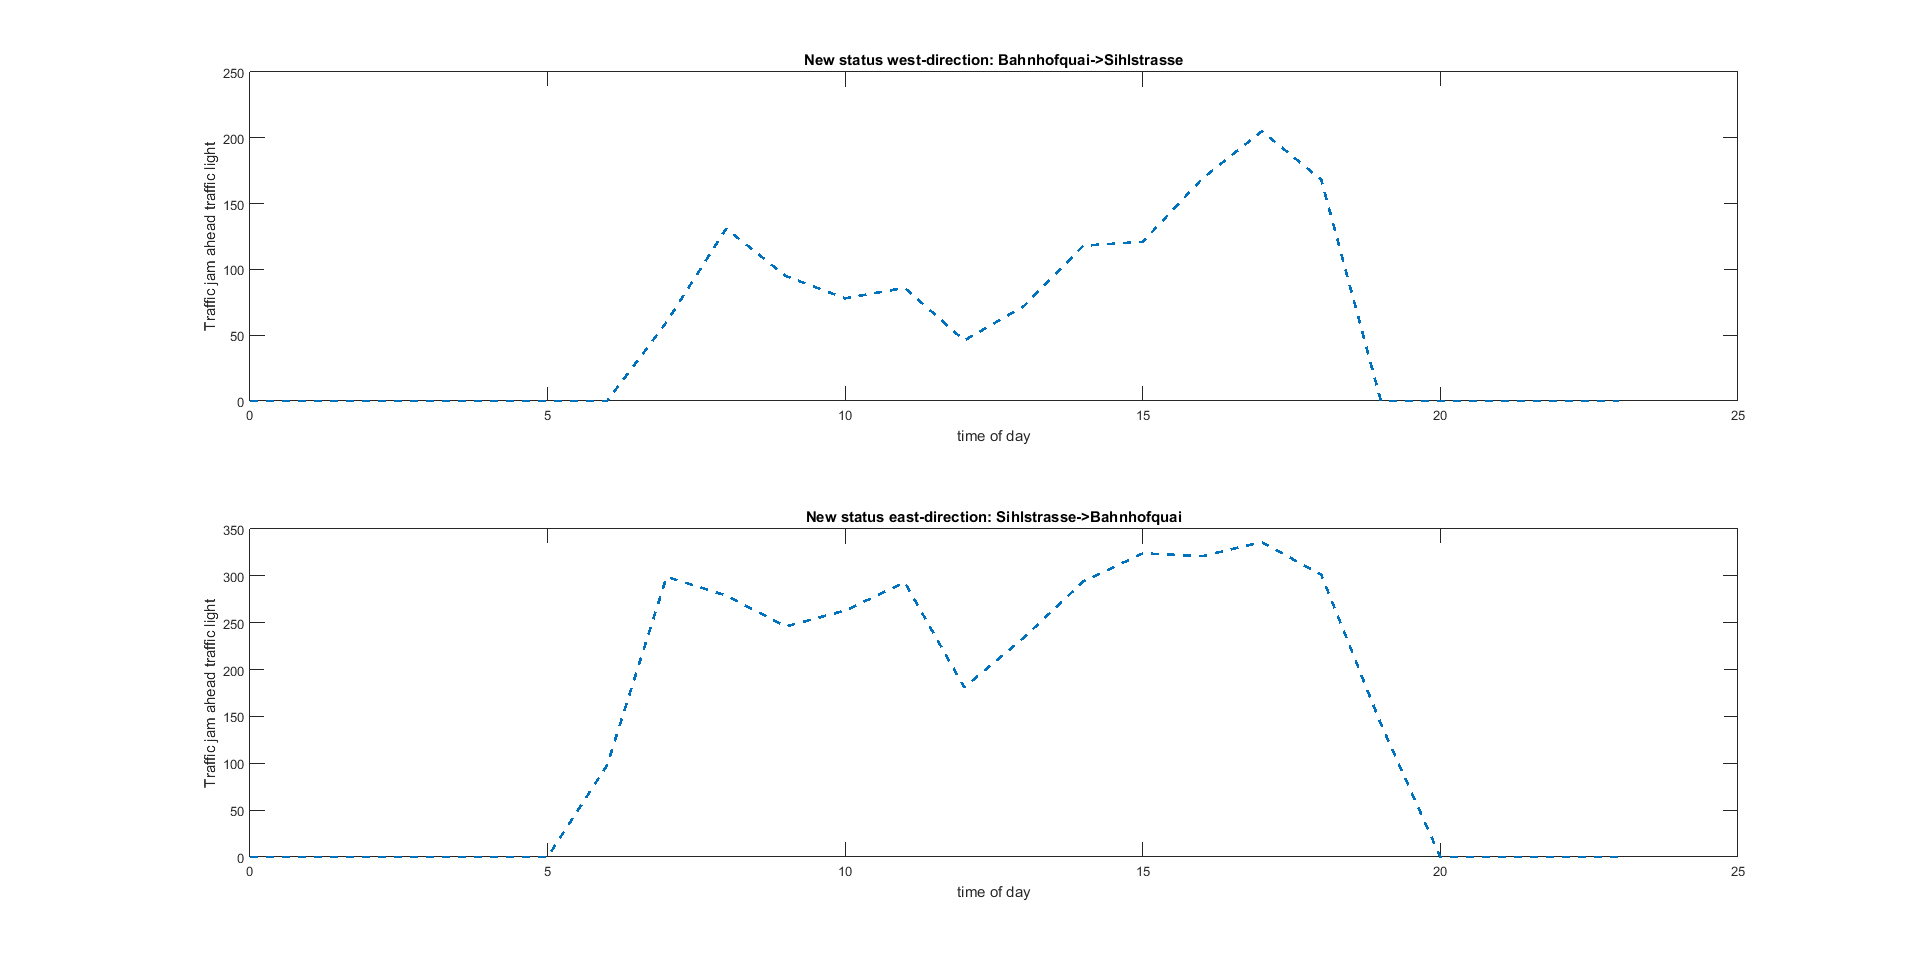
\includegraphics[width=\textwidth]{New_Traffic_jam.png}
\caption{This figure shows the traffic jam on a full 24h day for the one and two lane street (future status). One can see the traffic jam peaks in the morning hours and the evening hours. }
\label{traffic24_compare}
\end{figure}

\begin{figure}[h]
	\centering
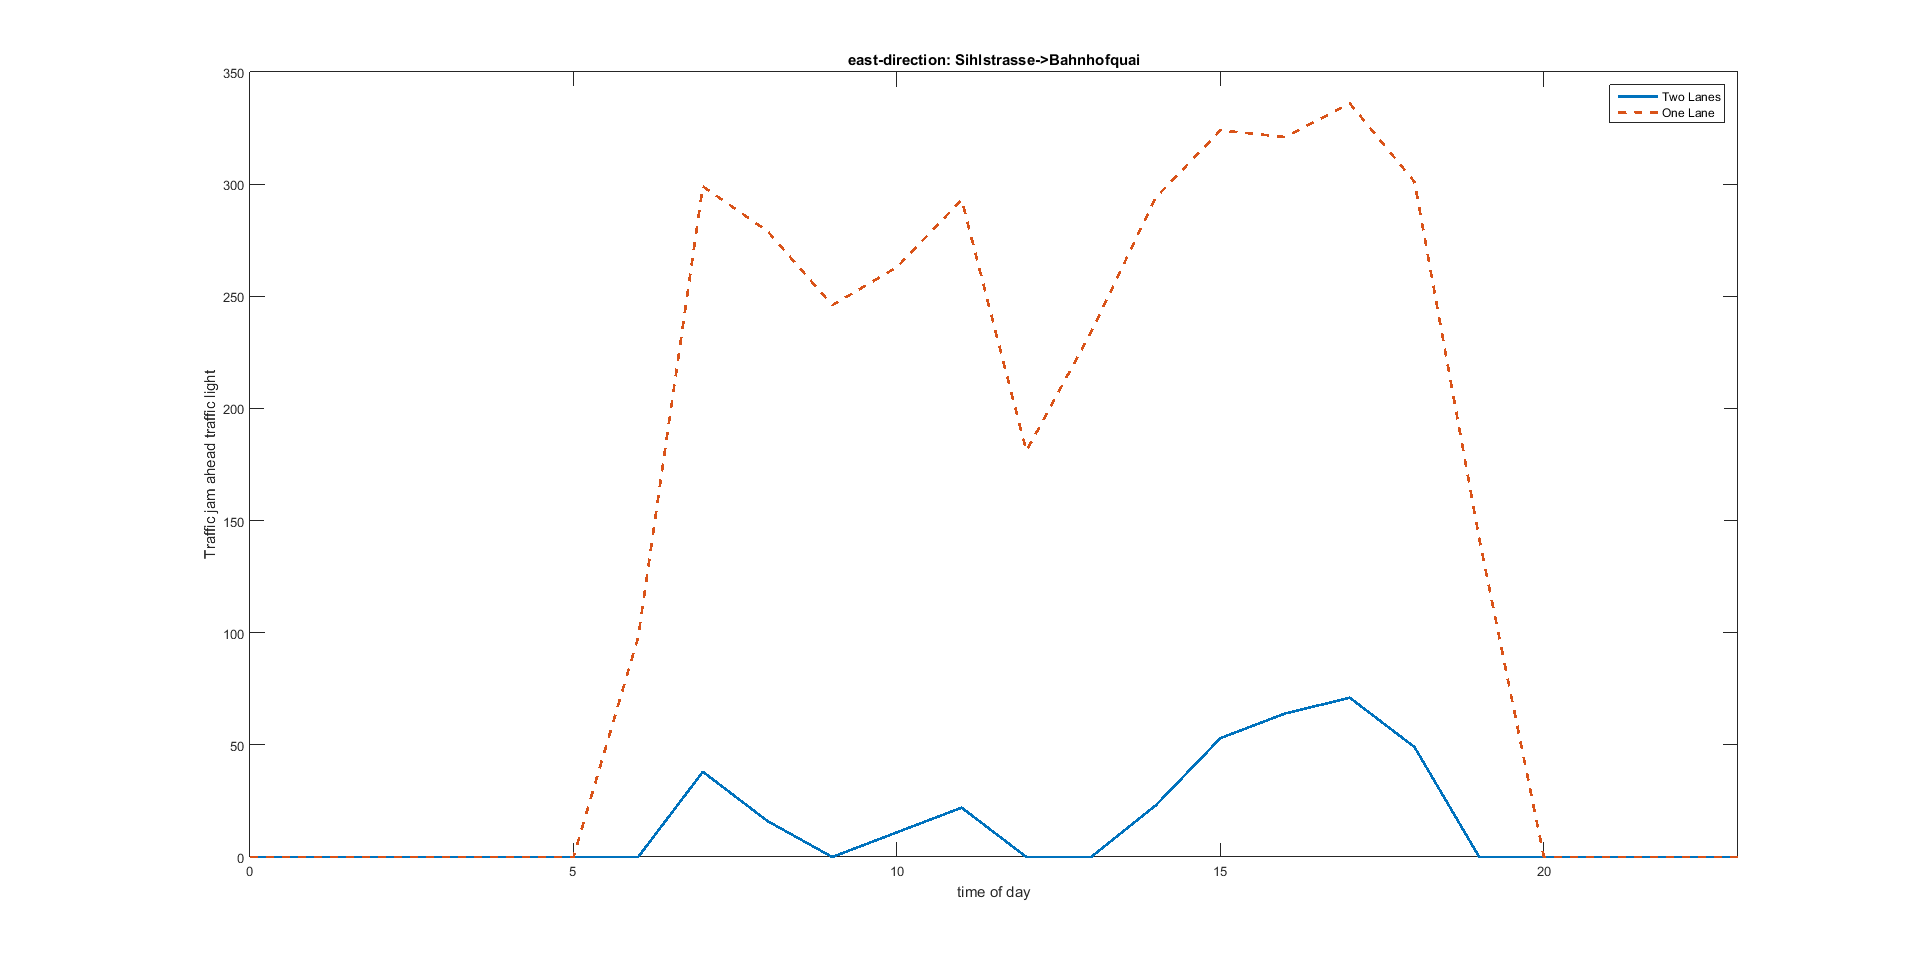
\includegraphics[width=\textwidth]{Comparison_Traffic_jam.png}
\caption{This figure shows the traffic jam on a full 24h day for the one and two lane street (future and current status) of the Sihlstrasse. One can see that the traffic jam is much higher with just one lane in this direction. }
\label{traffic24_1_lane}
\end{figure}
\begin{figure}[h!]
	\centering
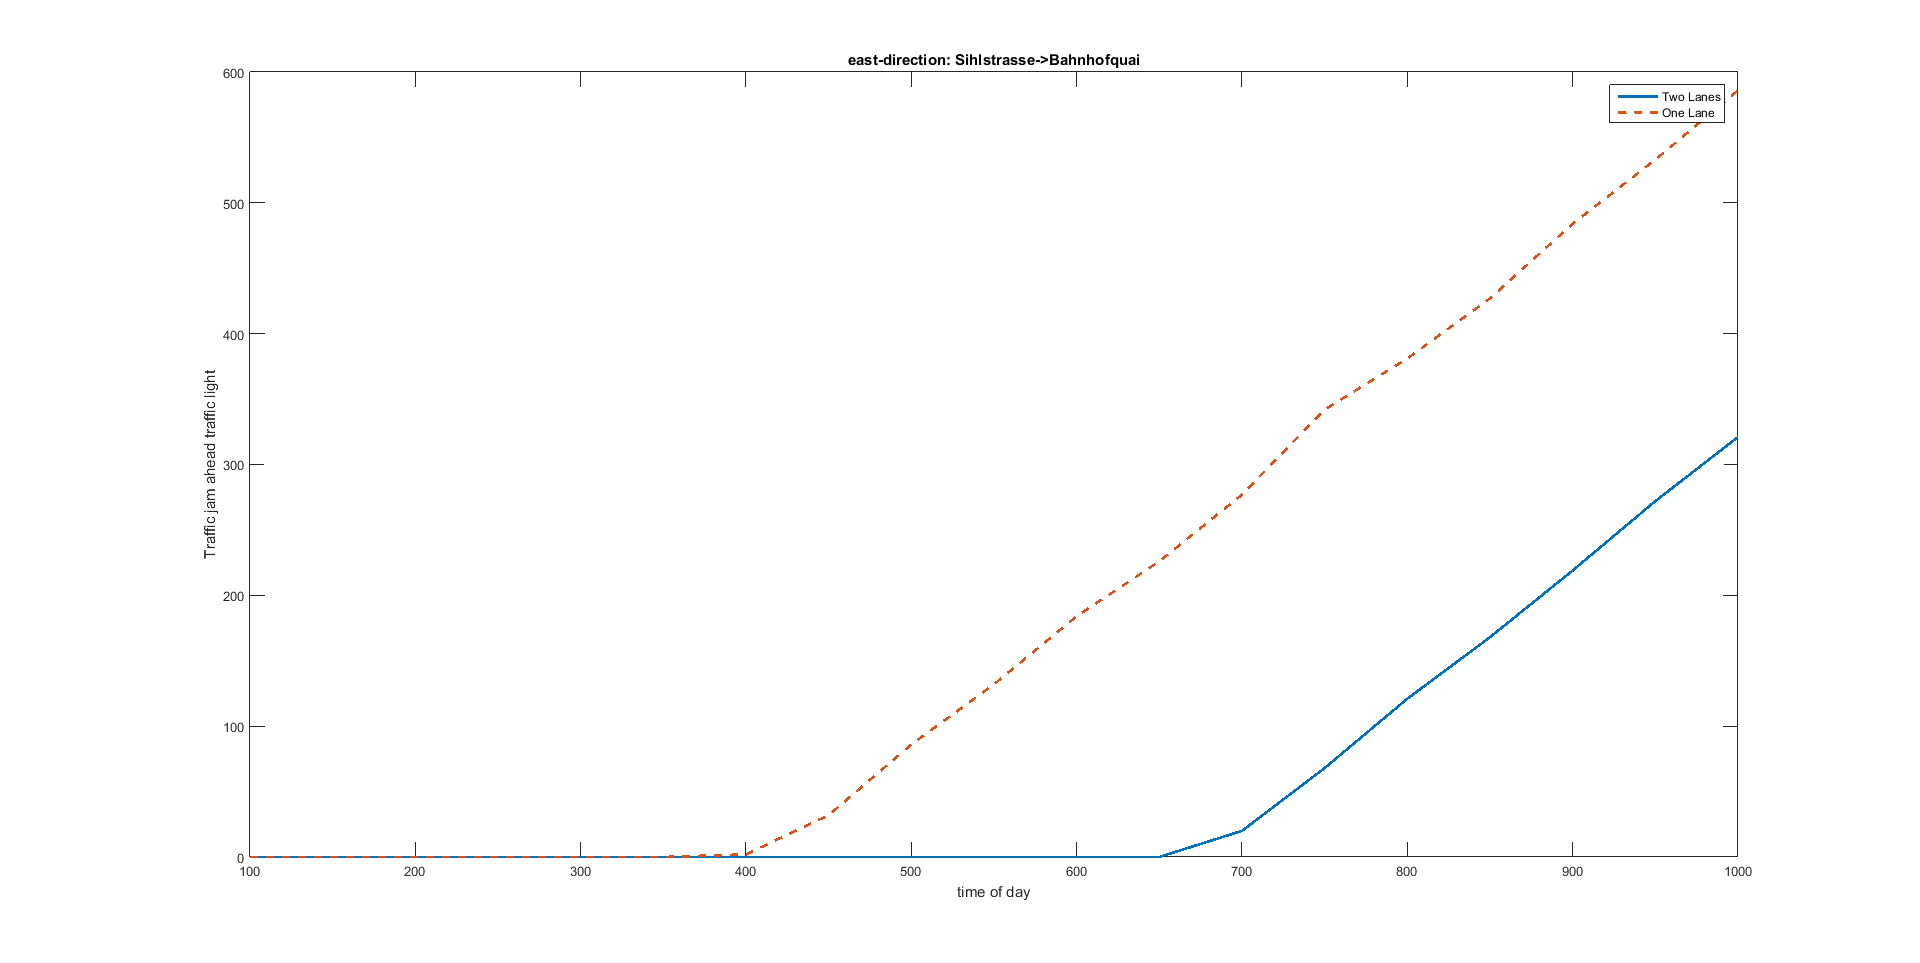
\includegraphics[width=\textwidth]{Comparison_Traffic_jam_1000.png}
\caption{This figure shows the traffic jam from 100 cars until 1000 cars per hour. }
\label{traffic24_carvolume}
\end{figure}


\section{Summary and Outlook}

In the project of the city of zurich \cite{project} the project manager wrote that they have to make some accompanying measures for the neighbourhood area. They do not give explicit suggestion how they look like. Our simulations shows that if they cancel one lane in direction east it will have a huge impact on the traffic jam. One have to handle a car volume which is 6 times higher than before. In our opinion they have to change a lot in this neighbourhood areas.\\
But to improve our model we should try to analyse what is the best set-up for the red and green cycle of the traffic lights. We think like this we can minimize the traffic jam.\\
Our simulation is very flexible, we can change all parameters very easily, therefore we can use it for different streets or different cities.

\newpage
\begin{thebibliography}{9}

\bibitem{project}
 Neue Verkehrsorganisation Uraniastrasse (project booklet),
 \emph{Tiefbauamt Stadt Zuerich,}
http://www.stadt-zuerich.ch/
  
\bibitem{theory}
 Physik des Straßenverkehrs,
 \emph{Andreas Schadschneider,}
 http://www.thp.uni-koeln.de
 
\bibitem{tief1}
 Tiefbauamt Stadt Zürich,
 \emph{Roland Frei,}
 Projektleiter Infrastruktur + Raum, roland.frei@zuerich.ch
  
\bibitem{tief2}
 Tiefbauamt Stadt Zürich,
 \emph{Gian Doenier,}
 Chef Verkehrssteuerung / Stv. L VM, gian.doenier@zuerich.ch
 
\end{thebibliography}

\newpage
\lstset{language=Matlab,%
    %basicstyle=\color{red},
    breaklines=true,%
    morekeywords={matlab2tikz},
    keywordstyle=\color{blue},%
    morekeywords=[2]{1}, keywordstyle=[2]{\color{black}},
    identifierstyle=\color{black},%
    stringstyle=\color{mylilas},
    commentstyle=\color{mygreen},%
    showstringspaces=false,%without this there will be a symbol in the places where there is a space
    numbers=left,%
    numberstyle={\tiny \color{black}},% size of the numbers
    numbersep=9pt, % this defines how far the numbers are from the text
    emph=[1]{for,end,break},emphstyle=[1]\color{red}, %some words to emphasise
    %emph=[2]{word1,word2}, emphstyle=[2]{style},    
}


\section*{Matlab Code}

\lstinputlisting{test_input.m}
\lstinputlisting{test.m}
\lstinputlisting{acceleration.m}
\lstinputlisting{slow_down.m}
\lstinputlisting{hang_behind.m}
\lstinputlisting{map_update.m}
\lstinputlisting{add_cars.m}
\lstinputlisting{add_one_car.m}
\lstinputlisting{change_traffic_light_sihlstrasse.m}
\lstinputlisting{change_traffic_light_uraniastrasse.m}
\lstinputlisting{output_bahnhofquai.m}
\lstinputlisting{output_sihlstrasse.m}
\lstinputlisting{simulation_sihlstrasse_new.m}
\lstinputlisting{simulation_sihlstrasse_one_line.m}
\lstinputlisting{simulation_uraniastrasse.m}


\end{document}  



 
